\documentclass[noback,landscape]{infposter}
\usepackage[utf8]{inputenc}           % Enables UTF-8 encoding
\usepackage{lipsum}
\usepackage{csquotes}
\usepackage{framed}
\usepackage{tikz}                    % Drawing trees
\usetikzlibrary{trees,shapes.multipart}
%% Checkmark
\def\checkmark{\tikz\fill[scale=0.4](0,.35) -- (.25,0) -- (1,.7) -- (.25,.15) -- cycle;}

% Source code listings
\usepackage{listings}

\lstset{
 backgroundcolor=\color{white},   % choose the background color; you must add \usepackage{color} or \usepackage{xcolor}
 basicstyle=\ttfamily\footnotesize,        % the size of the fonts that are used for the code
 keywordstyle=\bfseries,
 commentstyle=\itshape,
 % SL: lstinline doesn't work properly if breakatwhitespace is not set to true
 breakatwhitespace=true,         % sets if automatic breaks should only happen at whitespace
 breaklines=true,                 % sets automatic line breaking
 captionpos=b,                    % sets the caption-position to bottom
 escapeinside={\#*}{*\#},          % if you want to add LaTeX within your code
 extendedchars=true,              % lets you use non-ASCII characters; for 8-bits encodings only, does not work with UTF-8
 frame=none,	                   % adds a frame around the code
 keepspaces=true,                 % keeps spaces in text, useful for keeping indentation of code (possibly needs columns=flexible)
 numbers=none,                    % where to put the line-numbers; possible values are (none, left, right)
 rulecolor=\color{black},         % if not set, the frame-color may be changed on line-breaks within not-black text (e.g. comments (green here))
 showspaces=false,                % show spaces everywhere adding particular underscores; it overrides 'showstringspaces'
 showstringspaces=false,          % underline spaces within strings only
 showtabs=false,                  % show tabs within strings adding particular underscores
 tabsize=1,	                   % sets default tabsize to 2 spaces
 title=\lstname,                   % show the filename of files included with \lstinputlisting; also try caption instead of title
 caption={},
 belowcaptionskip=-1\baselineskip,
 xleftmargin=0.1\parindent,
 columns=fullflexible
}

\definecolor{darkgreen}{rgb}{0.000000,0.392157,0.000000}
\definecolor{violetred}{rgb}{0.815686,0.125490,0.564706}

% Define Links as a lst-language
\lstdefinelanguage{Links}{% 
  morekeywords={typename, fun, op, var, if, this, true, false, else, case, switch, handle, handler, shallowhandler, open, do, sig},%
  sensitive=t, % 
  keywordstyle=\color{red},
  emph={Comp,Player,Bool,Int,GTree,Cheat,Zero,Choose,Rand,Move,Winner,Take,Return,Get,Put,GameState,Alice,Bob,Fork,Yield,Spawn,Send,Recv,Stop,Candidate,Just,Nothing,PID,Maybe},
  emphstyle={\color{blue}},
  comment=[l]{\#},% 
  escapeinside={(*}{*)},%
  morestring=[d]{"}%
}

\newcommand{\textapprox}{{\fontfamily{ptm}\selectfont\texttildelow}}
\newcommand{\wildarrow}{\texttt{\textapprox{}>}}
% Links style
\lstdefinestyle{links}{
  basicstyle=\linespread{1.0}\ttfamily,
  language=Links,
  literate= {~>}{{\wildarrow}}1
}

\lstset{style={links}}

\title{Effective Concurrency without the Hassle}
\subtitle{Using Algebraic Effects and Handlers}
\author{Daniel Hillerström \normalsize{(Supervisors: Christophe Dubach (ICSA), Sam Lindley (LFCS), and Paul Patras (ICSA))}}
\email{daniel.hillerstrom@ed.ac.uk}
\homepage{http://homepages.inf.ed.ac.uk/s1467124}

\footer{%
  \resizebox{!}{\footerheight}{\includegraphics{logo_icsa.eps}}%
  \hfill %
  \resizebox{!}{\footerheight}{\includegraphics{logo_lfcs.eps}} %
  \hfill %
  \resizebox{!}{\footerheight}{\includegraphics{epsrc_colour.eps}} %
  \hfill %
  \resizebox{!}{\footerheight}{\includegraphics{cdt_pervasive_parallelism.eps}}%
}

\abstract{%
Algebraic effects and effect handlers provide a modular abstraction
for effectful programming.
%
They support user-defined effects, as in Haskell, in conjunction with
direct-style effectful programming, as in ML.
%
They also present a structured interface to programming with delimited
continuations.
}

\begin{document}
\makeposter

\section{Motivation and research hypothesis}
Approaches to concurrency and parallelism tend to be \emph{non-modular},
difficult to \emph{reason} about, and hard to \emph{control}.

\begin{center}
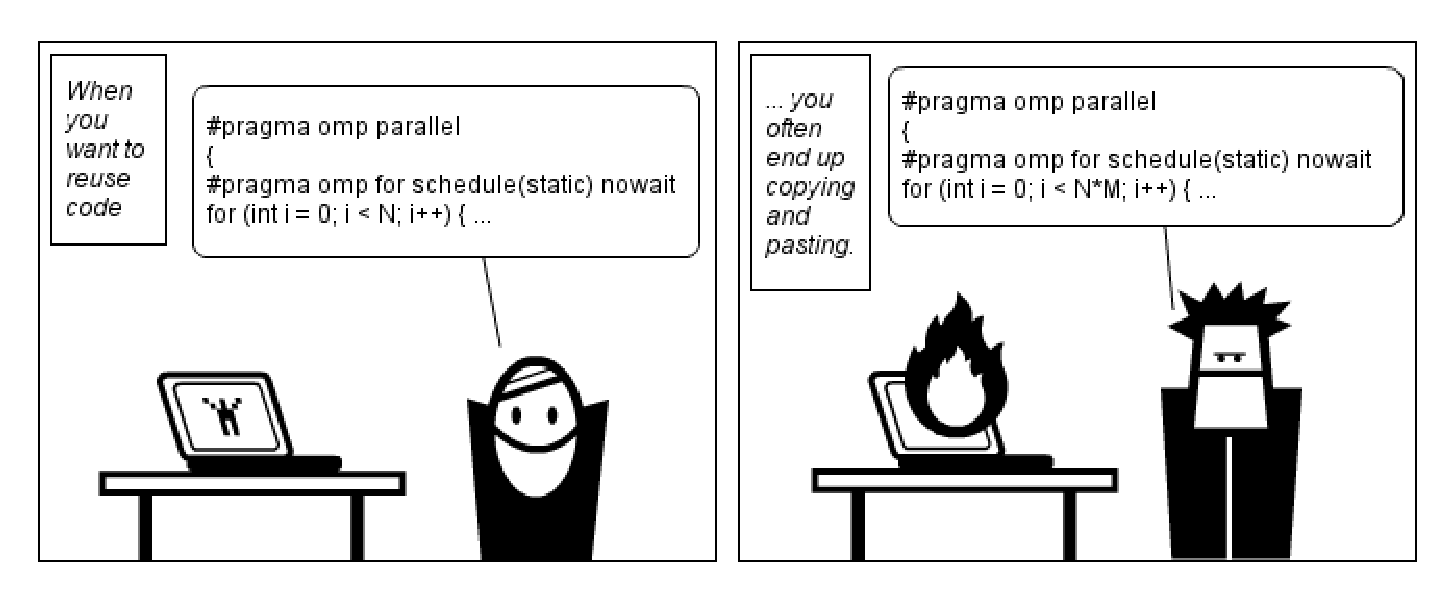
\includegraphics[scale=1.2]{reuse.eps}
\end{center}

\begin{center}
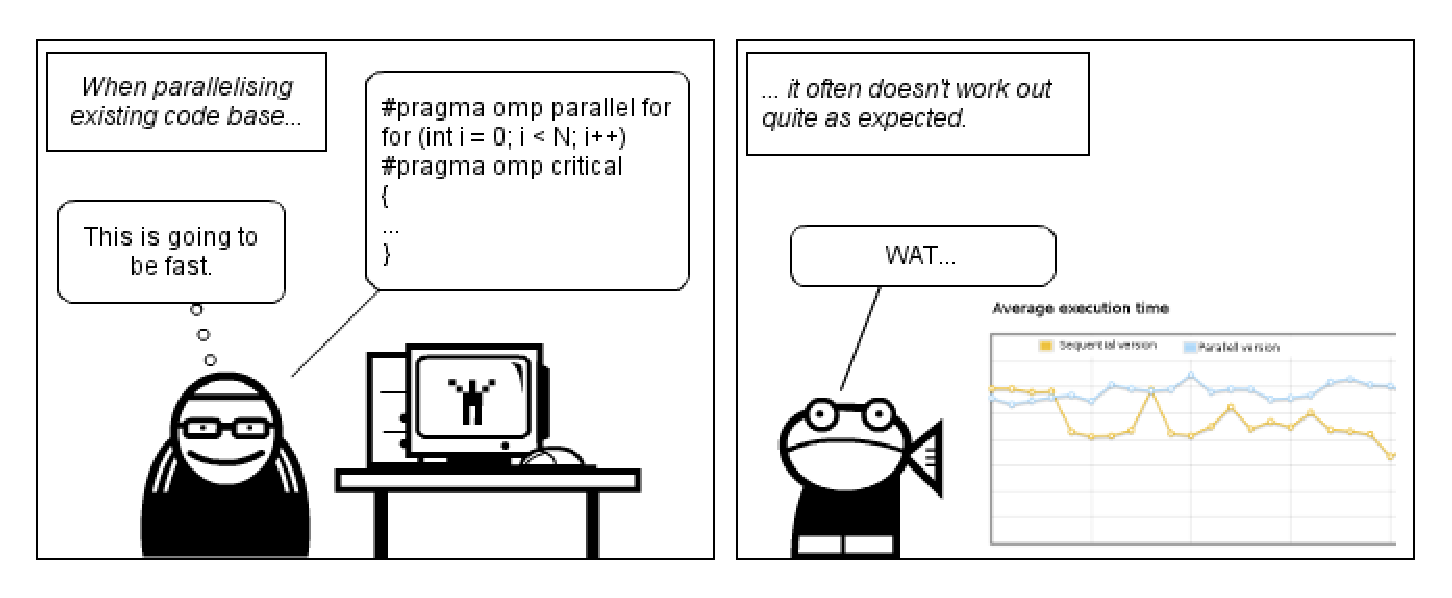
\includegraphics[scale=1.2]{wat.eps}
\end{center}

\textbf{Hypothesis} \emph{Reifying schedulers in the host programming
  language afford greater control, flexibility, and better means for
  reasoning.}
\section{Concurrency as an algebraic effect}
An algebraic effect is described by a collection of \emph{abstract} operations. For instance, we may describe concurrency by two operations:
\[
  \emph{concur} = \{\texttt{\lstinline$Spawn : ((PID) -> ()) \{\}-> PID$}, \texttt{\lstinline$Yield : ()$}\}
\]

Similarly, we may describe communication between processes:
\[
  \emph{comm} = \{\texttt{\lstinline$Send : (PID, a) \{\}-> ()$}, \texttt{\lstinline$Recv : (PID) \{\}-> Maybe(a)$}\}
\]
\vfill
\section{Scheduling processes}
A handler instantiates \emph{abstract operations} with concrete
implementations. For example, interpret $\emph{concur}$ as
co-operative processes:
\begin{lstlisting}[numbers=left]
fun run(proc)() {
 fun start(proc, pid) {
  handle(proc(pid)) {  # Start process with pid
   case Return(x)  -> 
    dequeue()()  # Process finished; run next process.
   case Spawn(child,k) -> 
    enqueue(fun() { k(pid+1) }); # Suspend parent process
    start(child, pid+1)          # Schedule child to run
   case Yield(k)   -> 
    enqueue(fun() { k(()) });    # Suspend process
    dequeue()()                  # Schedule another to run
 }}
 start(proc, 0)
}
\end{lstlisting}
\begin{description}
\item[Lines 2 and 3] begin the definition of a handler. The function
  \lstinline$start$ wraps the \lstinline$handle$ construct, which
  specifies how to interpret abstract operations through a sequence of
  clauses.

\item[Line 4] is a \emph{return clause}. It defines how to handle the
  final return value of the input computation. In this case, we
  dequeue the next process.

\item[Lines 5--9] are \emph{operation clauses}. They express how to
  handle \lstinline$Spawn$ and \lstinline$Yield$. In general, an
  operation clause takes the form $Op(p_1,\dots,p_n,k) \to M$, where
  $p_1,\dots,p_n$ are patterns that bind the operation parameters and
  $k$ is a pattern that binds the continuation of the computation in
  $M$.
\end{description}

The handler is described independently of the code (\lstinline$proc$)
it interprets.
\vfill

\section{Managing communication}
%A handler instantiates \emph{abstract operations} with concrete implementations. For example, we may interpret $\emph{comm}$ as a simple, global mailbox:
Similarly, we may interpret $\emph{comm}$ as a simple, global mailbox:
\begin{lstlisting}
fun mailbox(proc)() {
 handle(proc) {
  case Return(x)  -> x     # Forward return value
  case Send(to,data,k) ->  # Add message to message queue
    put((to, data) :: get()); 
    k(()) # k is the continuation of Send in proc
  case Recv(who,k) ->      # Take message from message queue
     var (msg,s) = lookup(who, get());
     put(s);
     k(msg) # k is the continuation of Recv in proc
} }
\end{lstlisting}

Communication is handled independently of process creation and the
application. We are free to choose the right method for the application.

% \section{Parallel prime number generation}
% % \begin{lstlisting}
% % fun generator(_)() {
% %   var n = 101; var first = pspawn(sieve);
% %   foreach([2..n], fun(p) { psend(first, Candidate(p)) });
% %   psend(first, Stop)
% % }
% % \end{lstlisting}
% We may express our concurrent or parallel applications independently
% of their actual interpretations. Consider a parallel version of \emph{Sieve of Eratosthenes}:
% \begin{lstlisting}
% fun sieve(mypid)() {
%  var myprime = fromCandidate(precv(mypid));
%  printInt(myprime);
%  fun loop(neighbour) {
%   switch (precv(mypid)) {  # Receive myprime
%    case Stop -> stop(neighbour)
%    case Candidate(prime) ->
%     if (prime `mod` myprime <> 0) { # Primality test
%      var neighbour =
%       switch (neighbour) { 
%        case Nothing   -> pspawn(sieve) # Spawn new process
%        case Just(pid) -> pid
%       };
%      psend(neighbour, Candidate(prime)); # Forward candidate
%      loop(Just(neighbour))
%     } else { loop(neighbour) }
%  } } 
%  loop(Nothing) }
% \end{lstlisting}

\section{Blocking modes}
Abstracting over the invocation of abstract operations gives us extra
flexibility. An interesting example is the invocation of
\lstinline$Recv$:
\begin{lstlisting}
sig bRecv : (PID) {Recv:(PID) {}-> Maybe(a),Yield:() |_}-> a
fun bRecv(me) {
  var m = do Recv(me); # Invoke Recv
  switch (m) {
    case Just(msg) -> msg
    case Nothing -> yield(); bRecv(me)
} }
\end{lstlisting}
The imperative \lstinline$do$ primitive invokes an abstract
operation. Notice, that we lift the message from being either
\lstinline$Nothing$ or \lstinline$Just(msg)$. This implementation
amounts to a blocking receive.

Given the signature of \lstinline$Recv$, it is easy implement a non-blocking receive: 
\begin{lstlisting}
fun nbRecv(me) { do Recv(me) }
\end{lstlisting}
% The invocation of the $\emph{concur}$ operations are straightforward:
% \begin{lstlisting}
% sig pSend : (Int,a) {Send:(Int,a) {}-> (),Yield:() |_}-> ()
% fun pSend(target, data) {
%   do Send(target, data); yield()
% }

% sig pSpawn : (a) {Spawn:(a) {}-> Int|_}-> Int
% fun pSpawn(f) { do Spawn(f) }

% sig pYield : () {Yield:() |_}-> ()
% fun pYield() { do Yield }
% \end{lstlisting}
% The imperative \lstinline$do$ primitive invokes an abstract operation.


% But abstracting over the invocation of operations gives us extra
% flexibility to implement different synchronisation modes. Here's an
% asynchronous send:


% The following implements a blocking receive:


% \section{Project overview}
% \begin{itemize}
%   \item Phase 1: Implement compiler for Links with effect handlers. $\checkmark$
%   \item Phase 2: Reconstruct Links' message-passing model. $\checkmark$
%   \item Phase 3: Implement and measure handler-oriented optimisations.
%   \item Phase 4: Add multicore support.
% \end{itemize}

% \section{Acknowledgements}
% This work is done in collaboration with OCaml Labs, Computer
% Laboratory, the University of Cambridge.

% This work was supported in part by the EPSRC Centre for Doctoral
% Training in Pervasive Parallelism, funded by the UK Engineering and
% Physical Sciences Research Council (grant EP/L01503X/1) and the
% University of Edinburgh.

% Supervisors: Christophe Dubach (ICSA) and Sam Lindley (LFCS).
\end{document}
